\section{Introduction}
This software is intended for use to calibrate, view, and analyze spectrum collected from various nuclear instrumentation. The document serves as the primary usage document. This software was developed using Python 3.8 and PyQt5 using packages such as Matplotlib and NumPy. The software has been developed into an executable file such that it can be run as any other program, this is done using PyInstaller. All code is considered open source. \\

This software is very much in beta phase testing, as such bugs and glitches are to be expeceted. You should report such bugs to the developer or care holder of the software upon discovery of such issues.

\section{Install and Initial Opening of Software}
This software is provided in a zip folder named Spectrum\_Viewer.zip, this folder contains all required libraries and packages for the software to run on a Windows configured machine. Before operation the software first must be unzipped, the built in method doing this in Windows10 should suffice. In the unzipped folder, there will be approximately 200 items. To easily locate the executable file, sort by file type and choose Application. The only file that should appear will be Spectrum\_Viewer.exe. This can be double clicked and the application will launch in full screen mode. \\

The interface will a window containing three main areas, shown below in Figure \ref{fig:opening}. The left most window will be populated when spectrum are being loaded. The right most window will be populated when spectrum are added to the graph. The center section features a full featured graphing utility. This graphing tool bar features the capabiltiy to zoom, pan, save, as well as other varius graphing features. It will be noted that the graph window appears to not fill the screen, this is corrected by navigating to the configure subplots selection. This will open a new dialog box, selection of ``Tight\_Layout'' will adjust the graph to full size. This may need to be repeated once spectrum are added. 

\begin{figure}[h!]
	\centering
	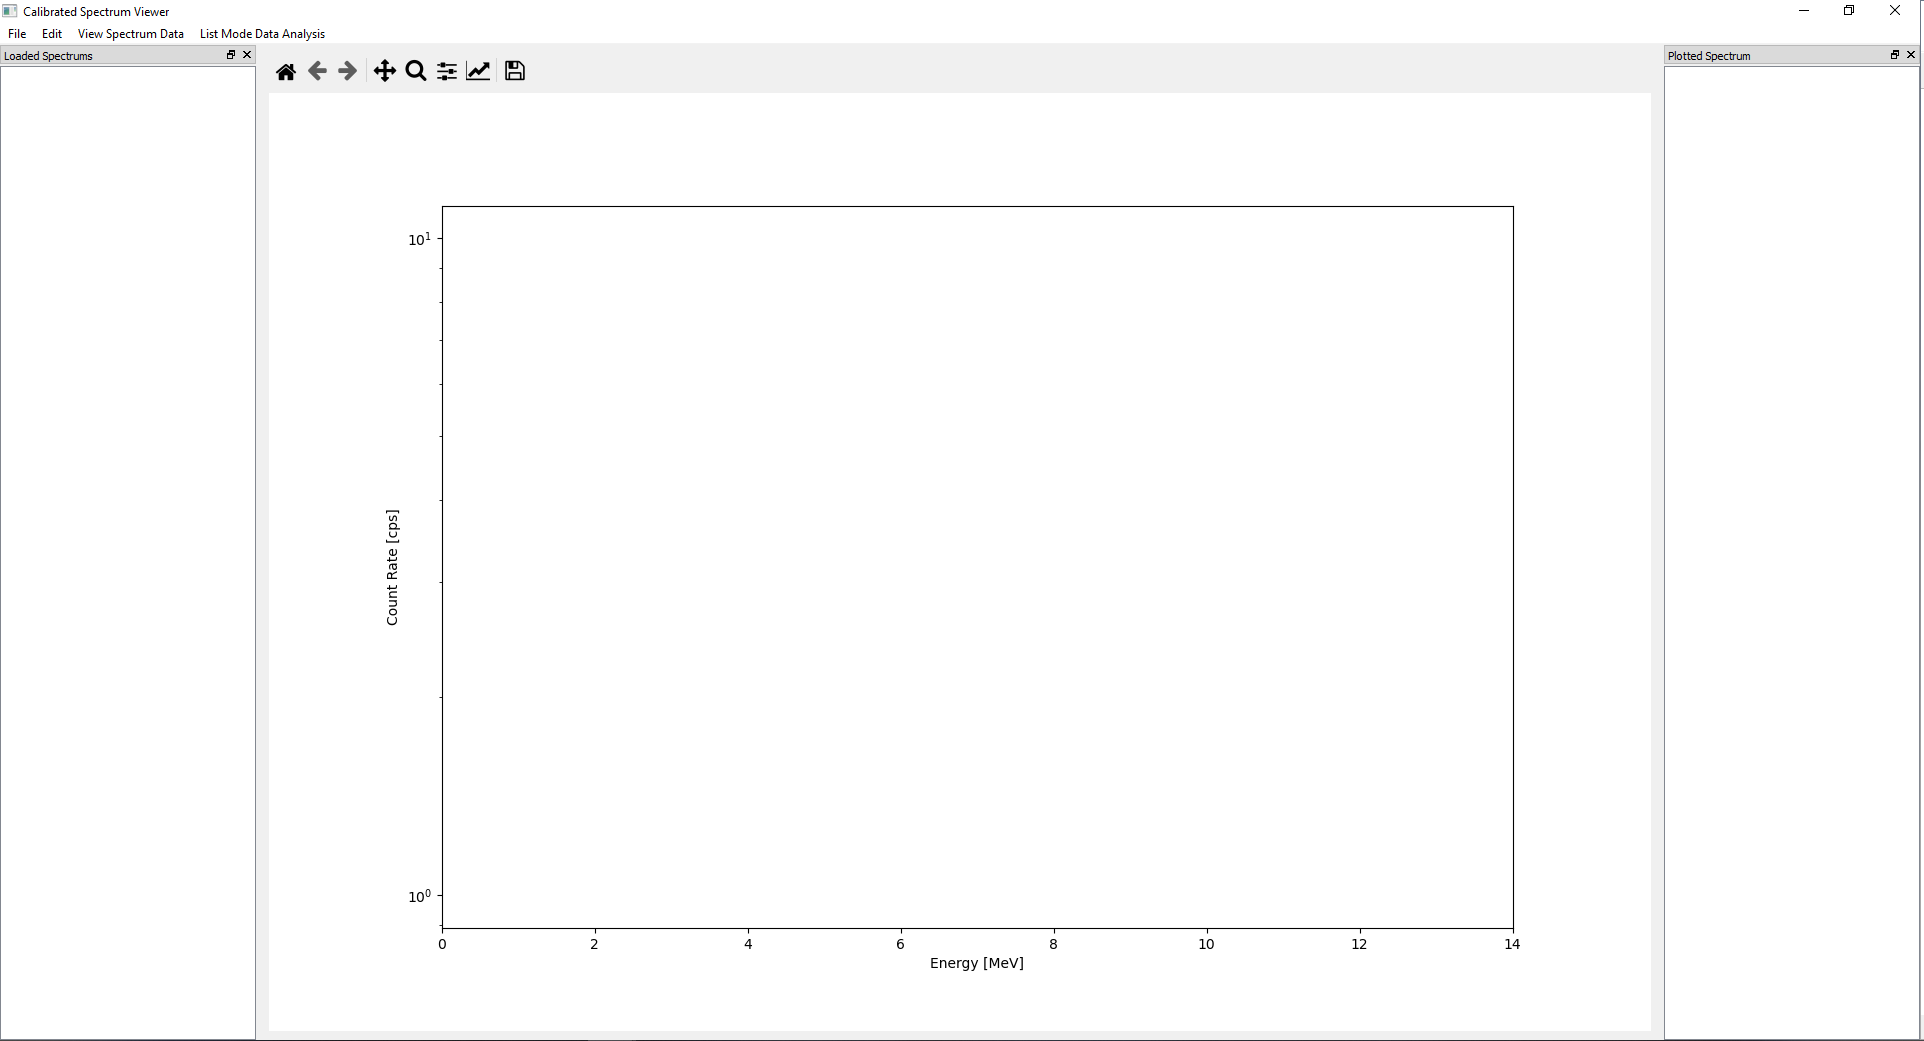
\includegraphics[width=\linewidth]{Front_Panel.png}
	\caption{User interface upon initial startup.}
	\label{fig:opening}
\end{figure}

\section{Discussion of Graph Setup}
The graph is initiated to be a energy calibrated, count rate spectrum. The count rate by default is shown in logarithmic scale to reveal small magnitude peaks. The energy by default ranges from 0 to 14MeV, the should encompass to vast majority of all possible energies normally seen, this can be adjusted, but more about that in a later section. 

